\subsection{DDF observing strategy}

In OpSim the choice to observe a given field is done on the fly according to an optimized selection function depending on criteria including (among others) observing conditions, slew time minimization, last time of visit, and total observing time. While the use of a simple metric (see below) would help in choosing another approach could be to use a pre-defined table that would specify which DDF are to be observed on a given night.

Let us consider the four reference fields \cosmos, \xmmlss, \cdfs~and \elais. Since the location are well known, it is possible to estimate when these fields are visible (that is with an altitude between 20 and 86.5 degrees) for a large enough period (typically 20 to 40 minutes) of good observing conditions (ie with airmass lower than a reference value - typically 1.5). We may define a (boolean) parameter dubbed observability equal to one when the above-mentioned conditions are filled, and 0 otherwise. This parameter is displayed on Figure \ref{fig:observability} (top). \xmmlss,\cdfs, and \elais~ are located in the same (Ra) region and may thus be observed during the same night whereas \cosmos~may be observed when all others are not visible. Season lengths of observability (Figure \ref{fig:observability} - bottom) range from 200 to 290 days.


\begin{figure}[!htbp]
\begin{center}
  
  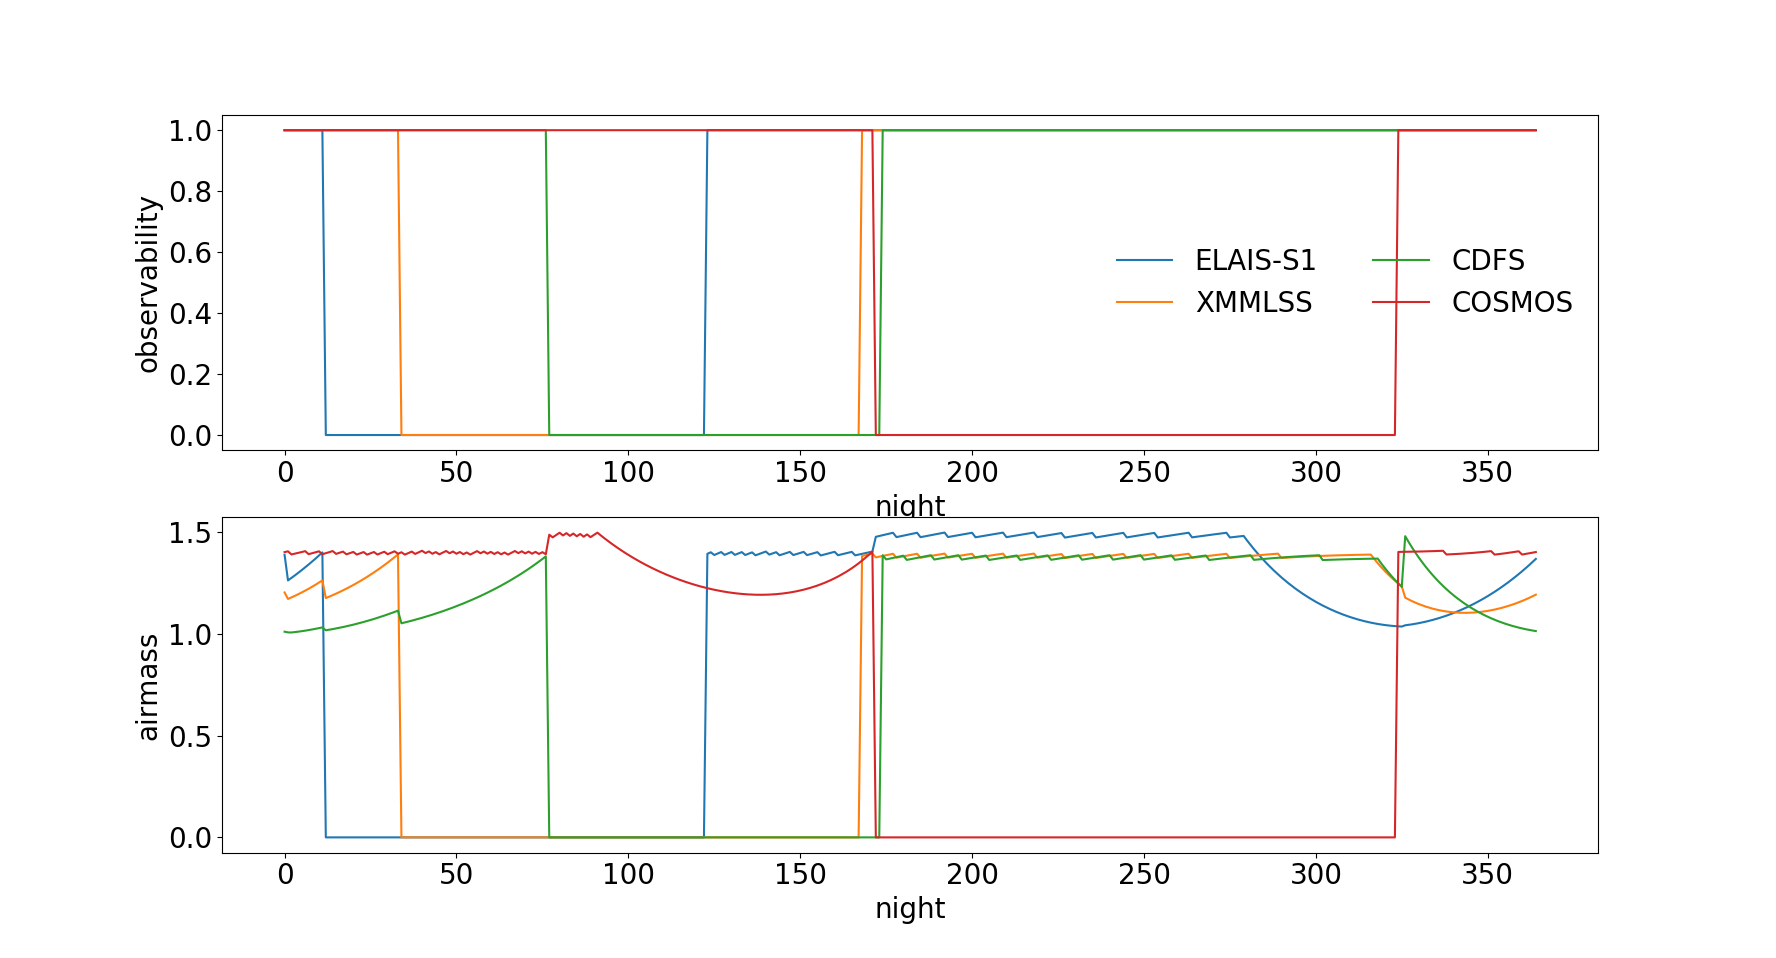
\includegraphics[width=18cm,height=12cm]{new_proposals/observability.png}
  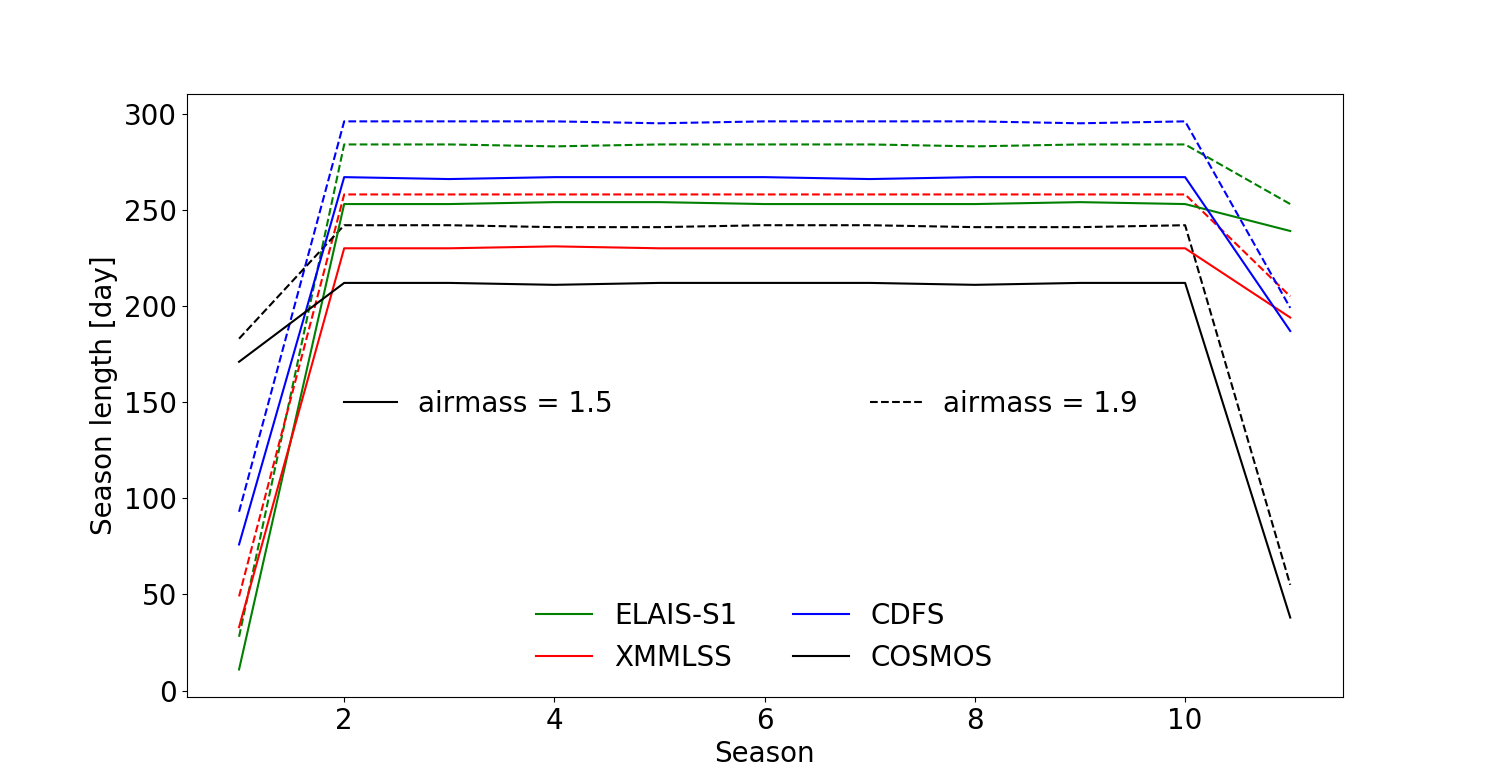
\includegraphics[width=18cm,height=8cm]{new_proposals/Season_length.png}
 \caption{Top: observability (see definition in the text) and airmass as a function of the night number (first year of LSST operation). Bottom: season length as a function of the season for an airmass limit of 1.5 (full lines) and 1.9 (dashed lines).}\label{fig:observability}
\end{center}
\end{figure}

The table of observations may be defined using median gap values \tgapcosmos~and \tgapothers~when \cosmos~and \xmmlss,\cdfs,\elais~are not observable, respectively. Observing time windows are then defined by:
\begin{itemize}
\item{[\tgapothers-w/2,\tgapothers+w/2]: \cosmos~ is observed}
\item{[\tgapcosmos-w,\tgapcosmos+w]: \xmmlss, \cdfs, \elais~are observed.}
\end{itemize}
with a width w equal to 2/3*(\tgapcosmos-\tgapothers).

\subsection{altsched rolling 80/20}

\subsection{altsched rolling 75/25}

\subsection{A simple metric for SN that may be implemented in OpSim/SLAIR}
If we fit a light curve model $L(t) = A \times \ell(t)$ on a
lightcurve $(t_i, y_i, \sigma_i)$, the least square estimate of $A$ is
given by:
$$
\hat{A} = \frac{\sum w_i \ell_i y_i}{\sum w_i \ell_i^2}
$$
and the signal-to-noise ratio on $\hat{A}$ is:
$$
SNR = \sum_i (w_i L_i^2)^{1/2}
$$ since we are in the background dominated regime, the weights may be
expressed as a function of the $5-\sigma$ limiting flux of each visit
$f_{i|5}$, and we have:
$$
SNR_{\mathrm{band}} = \sum_{i} 5 \times (f^{-2}_{i|5} L_i^2)^{1/2}
$$
where $5-\sigma$ limiting flux of each visit $f_{i|5}$.

This metrics is simple in the sense that it does not require to use a SN
light curve fitter. One just need lightcurve templates and the
limiting magnitudes of each visit -- given in the cadence
databases. In practice, using $SNR_g > 30, SNR_r > 40, SNR_i > 30$
(for $z<0.3$), and $SNR_r > 40$, $SNR_i > 30$ and $SNR_z > 20$ for
$z>0.3$ allows to fulfill the requirement on color resolution above.
